\documentclass[preprint,aps]{revtex4}
\usepackage{graphicx}

\newcommand{\ax}{{\bf a}_1}
\newcommand{\ay}{{\bf a}_2}
\newcommand{\Ax}{{\bf A}_1}
\newcommand{\Ay}{{\bf A}_2}

\begin{document}
\title{Packing Squares in a Torus}

\author{D. Blair}
\email[]{dwblair@physics.umass.edu}
\affiliation{Department of Physics,
University of Massachusetts,
Amherst, MA 01003-3720, USA}

\author{J. Machta}
\email[]{machta@physics.umass.edu}
\affiliation{Department of Physics,
University of Massachusetts,
Amherst, MA 01003-3720, USA}
\affiliation{Santa Fe Institute, 1399 Hyde Park Rd, Santa Fe, NM 87501, USA}

\author{C. Santangelo}
\email[]{santangelo@physics.umass.edu}
\affiliation{Department of Physics,
University of Massachusetts,
Amherst, MA 01003-3720, USA}

\begin{abstract}
The densest packings of $N$ unit squares in a torus are studied using analytical methods as well as simulated annealing.  A rich array of dense packing solutions are found: density one packings when $N$ is the sum of two square integers; a family of ``gapped bricklayer'' Bravais lattice
 solutions with density $N/(N+1)$; and some surprising non-Bravais lattice configurations, including lattices of holes as well as a configuration for $N=23$ in which not all squares share the same orientation.  The entropy of some of these configurations and the frequency and orientation of density one solutions as $N \rightarrow \infty$ are discussed.

\end{abstract} 
\maketitle
\section{Introduction}

Understanding the dense packings of hard particles has yielded essential insights into the structure of materials \cite{Bernal2007} \cite{Zallen1983} \cite{Torquato2002} \cite{Chaikin2000}, granular media \cite{Torquato2002} \cite{Mehta1994}, number theory \cite{Cohn2008} \cite{Conway1999}, biology 
%\cite{Liang2001}
\cite{Gevertz2008} \cite{Purohit2003}, and computer science \cite{Johnson1974} \cite{Lodi2002}. This understanding has been hard won: millennia can elapse between a conjecture and its proof. This is best exemplified by sphere packing, for which a proof had not been found until 1998 \cite{Hales2011}.

%Note: for references in this above paragraph, see paper by Torguato and Jiao

% Note: I changed this from 1999 to 1998, given http://en.wikipedia.org/wiki/Thomas_Callister_Hales and other sources
Recent experimental advances have allowed the development of (nearly) hard colloids that, for entropic reasons, manifest the densest sphere packing [REF??]. The attempt to obtain a deep understanding of liquid crystal mesophases has suggested study of the dense packing of anisotropic particles. This has led to recent explorations of the packing of ellipsoids \cite{Donev2004}, polyhedra \cite{ROAN} \cite{BAKER}, and polygons \cite{Jansson2006} \cite{STROOBANTS}.

One of the simplest regular polygons one can pack in two dimensions is the square. On the plane, the densest packing is trivial -- a square lattice of squares. Monte Carlo simulations of squares at finite pressure, however, have also found a tetratic phase \cite{Donev2006b}, and experiments with hard colloidal squares have found, rather than the tetratic phase, a rhombic crystal having a different symmetry than the square \cite{Zhao2011}. Even the dense packing of a finite number of squares can be more complicated than naive considerations would indicate -- in fact, this problem has been shown to be NP-hard \cite{Leung1990}. The densest known packings of squares inside a larger square can be quite complex \cite{ERDOS1975} \cite{Friedman2002} when the number of squares is not a perfect square. Higher packing densities than that of a simple, square lattice with defects can be achieved through configurations in which some of the squares are rotated and shifted with respect to the simple square lattice \cite{Friedman2002}.

In this paper, we study an even simpler packing problem: finding the densest packings of squares in a torus -- that is, a larger square with periodic boundary conditions. Even with the additional translation symmetry afforded by packing squares in a torus rather than in a square, the resulting dense packings in the torus can still be far from simple. As in many other mathematical packing problems, the strategy here is to search for the smallest area torus that can accommodate a fixed number of squares $N$.  We use a combination of analytic and Monte Carlo simulated annealing techniques to accomplish this, and our results can be summarized as follows: we find that whenever $N$ can be expressed as the sum of two integers -- $N=n_1^2+n_2^2$ -- the densest possible packing is a density one packing with squares arranged in rows that are at an orientation of tan$^{-1}(n_2/n_1)$ relative to the underlying torus.  For other cases of $N$ up to $N=27$, we find a surprisingly rich collection of dense packing structures. For $N$ = 6,11,14, and 27, we believe that the optimal packing is also a commensurate Bravais Lattice packing with density $N/(N+1)$ and resembles a bricklayer pattern with periodic gaps.  For $N=$ 12,21,22 and 23, we find that the densest configurations are non-Bravais lattice packings, including both regular lattices of holes and of skewed squares. These results are summarized in Table I within Section II.

In Section II, we present a summary analysis of the various structures we found for $N$ up to 27, including both commensurate Bravais lattice solutions and non-Bravais lattice solutions.  The packing motifs we found through analytic and numerical means are illustrated in this section via both drawn figures and images generated by our numerical simulations. In Section III, we provide details of our numerical experiments for the hard square system. Section IV is a discussion of our results, including an analysis of the entropy of density one packings and the rotational invariance of such packings as $N \rightarrow \infty$. [DOES THIS LAST SENTENCE WORK?]


\section{Analysis of Packings}
\label{sec:analytics}

In this section we give an analytic treatment of square packings on a torus.  We first describe a set of solutions in which the squares lie on a Bravais lattice, and then turn to more complicated cases. The density one solutions are optimal by construction, and all of the other solutions are conjectured to be optimal. The numerical results of Sec. \ref{sec:numerical} guided us to the conjectured solutions, and the fact that long simulated annealing runs consistently produced these solutions gives us some confidence that they are optimal.  Our conjectures for the first 27 values of the number of squares are summarized in Table \ref{table}.

\subsection{Commensurate Bravais Lattice Solutions}
Here we consider a class of Bravais lattice configurations that includes all of the density one packings and other solutions we have found for  $N \leq 27$.   In all of these packings the squares are lined up in rows.  For the purpose of this analysis, we assume these rows are aligned along the x-axis. Thus one of the primitive vectors of the lattice of squares is $\ax=\hat{{\bf x}}$.   The second primitive vector is taken to have the form $\ay=c \hat{{\bf x}} + d \hat{{\bf y}}$ with $-1< c <1$ and  $d\geq 1$.  The primitive vectors of the torus, $\Ax$ and $\Ay$, need not be aligned with the primitive vectors of the squares.     The requirement that the squares pack periodically on the torus is equivalent to saying that the lattice of squares is commensurate with the larger square lattice of the torus.  That is, there exist  integers $n_1$, $n_2$, $n_3$ and $n_4$ such that the torus primitive vectors $\Ax$ and $\Ay$ are given by
\begin{eqnarray} 
\label{eqn:Ana}
\Ax&=& n_1 \ax + n_2 \ay \nonumber \\ 
\Ay&=&n_3 \ax + n_4 \ay.
\end{eqnarray}
In addition, we require that the torus primitive vectors are of equal length,
\begin{equation}
\label{eqn:normal}
|\Ax|=|\Ay| ,
\end{equation}
and orthogonal,
\begin{equation}
\label{eqn:ortho}
\Ax \cdot \Ay = 0 .
\end{equation}
[ COMMENTS? ] [ HOW DO WE RECONCILE C>0 WITH FINITE ENTROPY OF PERFECT SQUARE PACKING?]
These conditions are uniquely solved by
\begin{eqnarray}\label{eq:gap}
c &=& - \frac{n_1 n_2 + n_3 n_4}{n_2^2 + n_4^2}\\
d &=& \frac{| n_1 n_4 - n_2 n_3|}{n_2^2 + n_4^2} \nonumber
\end{eqnarray}
The number of squares $N$ packed on the torus is the number of lattice points of the squares lattice in a unit cell of the torus lattice
\begin{equation}
\label{eqn:N}
N = |n_1 n_4 - n_2 n_3|,
\end{equation}
and the areal density of the squares $\rho$ is given by
\begin{equation}
\label{ }
\rho=N/|\Ax \times \Ay| = 1/d.
\end{equation}

\subsubsection{Density one packings}
There are two classes of density one solutions.  The first is the perfect square packing.  Here $c=0$, $d=1$, $n_1=n_4=\sqrt{N}$ and $n_2=n_3=0$.  This simple packing is shown in Fig. \ref{fig:N9} for the case of $N=9$.  Note that on the torus, each of the $n_1$ rows (or columns, but not both) may be arbitrarily displaced relative to the other rows (columns) without disturbing density of the packing or its periodicity.  Thus, the perfect square packings have finite entropy.

There is a more general class of density one packings for which the lattice of squares may be tilted with respect to the primitive vectors of the torus. Setting $d=1$ and $c=0$ in Eq. (\ref{eq:gap}), we find $N=n_2^2 + n_4^2$, $n_1=-n_4$, and $n_2 = n_3$.  The perfect square solution is the special case $n_2 = n_3 = 0$, with the square lattice oriented at an angle of $\tan^{-1}(n_2/n_1)$ relative to the torus lattice vectors.   Clearly, these density one, tilted square lattice solutions are optimal for all $N$ that are sums of two square integers.  Fig. \ref{fig:bravais} shows the case $N=10$ ($n_1=3$ and $n_2=1$).

The packing has density one if and only if $N$ is a sum of two squares; and the converse of this is also true: $N$ is a sum of two squares whenever we have a density one packing of squares in the torus. To prove this, first note that every square in a $\rho=1$ packing must have at least four other squares bordering it along a finite segment length, forcing all $N$ squares to share the same orientation.  Now consider three squares in mutual contact with each other, a configuration that must exist if the packing has no gaps. Two of those squares must be aligned in a row, as shown in Fig. \ref{fig:aligned}. In order to eliminate gaps in the packing, those three squares define a set of rows that the entire packing must respect. The periodicity of periodic boundary conditions on a set of rows now ensures that $N$ can be [????] expressed as $n_2^2 + n_4^2$ via the Pythagorean theorem (see Fig. \ref{fig:gb}).

\subsubsection{Density one packings with defects}

The simplest way to produce candidates for a densest packing for $N=n_2^2 + n_4^2$ is to remove $k$ squares from a density one packing; indeed, our numerical results suggest that for several values of $N$, the optimal packing is a density one packing configuration with one missing square.  This is indicated in the `Comment' column in the Table using the notation $n_1^2-k$ or $n_1^2+ n_2^2-k$ depending on whether they are generated by removing $k$ squares from $N$ a square integer or a sum of two square integers respectively. Examples include $N=3$, $7$ and $15$. Note that these configurations have finite entropy since the hole(s) in the lattice can be distributed arbitrarily.

[ should the notation $n_1^2-k$ or $n_1^2+ n_2^2-k$ include a -1??? or ...? For $N \leq 27$, $k=1$] (see jon's edits]

%Although for small $N$, the density of sums of two squares together with perfect squares is relatively high,  it is known RAMANUJAN ETC REFERENCE that these values of $N$ have vanishing density among all positive integers. In particular the density of sums of two squares less than $n$ behaves asymptotically as $1/\sqrt{\log(n)}$. One interesting consequence of this is that $\rho=1$ packings appear with vanishing frequency as $N  \rightarrow \infty$. 

%Unlike the perfect square packings, the sum of two squares packing must have all the rows of squares aligned and do not have finite entropy.

\subsubsection{Bricklayer packings with gaps}
Next we consider Bravais lattice solutions that have density less than one -- that is, $d>1$.  Because these solutions may also have rows that must be shifted relative to one another ($c\neq 0$), we call these `gapped bricklayer configurations.'  An example is shown in Fig. \ref{fig:gb}(a).  The equations of (\ref{eq:gap}) allow us to ennumerate all gapped bricklayer configurations. Since the packing density of these configurations is $(n_2^2 + n_4^2)/N$, the highest packing density we can find within this class of configurations with density less than unity must numbers of the form $n_2^2 + n_4^2 = N-1$.  This requires that $N$ be one more than a sum of two squares. The first several are 2,3,6,11,14,18,26, and 27.  Based on the numerics we believe that for $N=6$, 11, 14 and 27, the gapped bricklayer packing is optimal. These are indicated in the Table with the abbreviation `GB' in the Comment column. The associated (not unique) lattice vectors are shown in the rightmost columns of the Table for the GB packings.  There are also gapped bricklayer solution for density $(N-2)/N$ when $N$ is two more than a sum of two squares though we have not found any candidate optimal solutions of this form for $N \leq 27$. Unlike the bravais lattice packings with density one, different rows of the gapped bricklayer solutions have a fixed shift given by $c = - (n_1 n_2 + n_3 n_4)/(n_2^2 + n_4^2)$. The denominator is the closest sum of two squares below $N$. 

\subsection{Non-Bravais Lattice Packings}

Here we consider special cases suggested by our numerical simulations that do not correspond to Bravais lattice packings.
Note: if the 'Comment' column of the Table simply repeats a value of $N$, it indicates a special case for which the squares are not on a Bravais lattice and for which there is not an obvious pattern that can be extrapolated easily to optimal packings for higher values of $N$.

\subsubsection{Gapped bricklayer with domino bricks, $N=22$}
The conjectured best packing for $N=22$ is shown in Fig. \ref{fig:n22} It is actually a gapped bricklayer configuration except that the unit cell or brick is composed of two squares stacked in the $\hat{{\bf y}}$ direction (the direction perpendicular to the rows).  Except for this difference, the configuration is identical to the $N=11$ gapped bricklayer and has density $\rho= 10/11$.

\subsubsection{Lattice of $\frac{1}{2}\times\frac{1}{2}$ holes, $N=12$ and $23$}
The conjectured best configurations for $N=12$ and 23 are shown in Figs. \ref{fig:n12} and \ref{fig:n23}, respectively.  In both cases the motif can be described as a lattice of $\frac{1}{2}\times\frac{1}{2}$ holes. It is straightforward to verify that these motifs are in fact packings on the torus and have the density $N/(N+k/4)$ where $k$ is the number of holes in the unit cell.  For $N=12$, evidently $k=2$ and for $N=23$, $k=5$. 


\subsubsection{Lattice of skew squares embedded in a square lattice, $N=21$}
The conjectured densest packing for  $N=21$, shown in Fig.\ \ref{fig:n21}, does not follow any of the motifs described heretofore. The unit cell consists of a $4 \times 4$ square with motif of 5 squares attached to its side.  This 5-square pattern is also the best packing of 5 squares in a square \cite{Friedman2002}.  A simple calculation yields the density, $\rho= 21/(4^2+(2+1/\sqrt{2})^2)$.  This packing has one square per unit cell tilted at 45$^{\circ}$ relative to all other squares.  This is the only example that we found for which not all of the squares in the motif are oriented in the same way. It was also the most difficult configuration for our simulated annealing algorithm to find. 

\subsection{Table of Results}

To summarize: the perfect square, sum of two squares and gapped bricklayer configurations cover most of the case we have found for $N \leq 27$.  The Table gives optimal configurations (if $\rho=1$) and conjectured optimal configurations (if $\rho<1$), for each value of  $N$ less than 28.  The column `$\rho$' is the density of the configuration. The `Comment' column describes the type of lattice.   For example, $3^2$ indicates a perfect square and $5^2-1$ indicates a perfect square with one square missing.  Similarly $3^2+1^2$ refers to the sum of two squares and `GB' stands for `gapped bricklayer.'  If a single number is in the `Comment' column it refers to one of the special cases discussed above.  The four columns `$n_1$, $n_2$, $n_3$, $n_4$' are shown if the configuration of squares is itself a Bravais lattice and these integers are the coefficients of the lattice vectors of the torus in terms of the lattice vectors of the squares as defined in (\ref{eqn:Ana}).  Only those columns needed to specify the lattice are filled in.

\vspace{.3in}
\begin{table}
\label{table}
\caption{Exact and conjectured densest packed configurations of squares on a torus.  Refer to the text for the meaning of the columns.}
  \begin{tabular}{|c | c|c | c| c | r | c | c | c |}
\hline
% after \\ : \hline or \cline{col1-col2} \cline{col3-col4} ...
  $N$ &$\rho$&Comment& $n_1$ & $n_2$ & $n_3$ & $n_4$  \\ \hline \hline
   1 &1&  $1^2$ & 1&  &   &    \\ \hline 
   2 &1&  $1^2+1^2$ &1& 1 &  &  \\ \hline
   3 &$3/4=0.75$&  $2^2 -1$ &2&  & &   \\ \hline
   4 &1&  $2^2$ &2& & &   \\ \hline
   5 &1&  $2^2+1^2$ &2& 1 &    & \\ \hline
   6 &$5/6=0.8\bar{3}$& GB &2& -1 &2 & 2   \\ \hline
   7 &$7/8=0.875$& $2^2+2^2 -1$ &2& 2 & &     \\ \hline
   8 &1& $2^2+2^2 $ &2& 2 & &     \\ \hline
   9 &1&  $3^2$ &3& & &  \\ \hline
   10 &1&  $3^2+1^2$ &3& 1 &    & \\ \hline
   11 &$10/11=0.\overline{90}$& GB &3& 1 &-2 & 3   \\ \hline
   12 &$24/25=0.96$& 12 && & &    \\ \hline
   13 &1&  $3^2+2^2$ &3& 2 &    & \\ \hline
   14 &$13/14=0.9\overline{285714}$& GB &3& 2 &4 & 2   \\ \hline
   15 &$15/16=0.9375$&  $4^2 -1$ &4&  & &   \\ \hline
   16 &1&  $4^2$ &4& & &   \\ \hline
   17 &1&  $4^2+1^2$ &4& 1 &    & \\ \hline
   18 &1&  $3^2+3^2$ &3& 3 &    & \\ \hline
   19 &$19/20=0.95$&  $4^2 +2^2 -1$ &4& 2 & &   \\ \hline
   20 &1&  $4^2+2^2$ &4& 2 &    & \\ \hline
   21 &$21/(4^2+(2+1/\sqrt{2})^2)=0.900189 \ldots$&  $21$ & &  &   &    \\ \hline 
   22 &$10/11=0.\overline{90}$& 22 &3& 1 &-2 & 3  \\ \hline
   23 &$92/97=0.94845 \ldots$&  $23$ & &  &   &    \\ \hline
   24 &$24/25=0.96$&  $5^2 -1$ &5&  & &   \\ \hline
   25 &$1$&  $5^2$ &5&  & &   \\ \hline
   26 &1&  $5^2+1^2$ &5& 1 &    & \\ \hline
   27 &$26/27=0.\overline{962}$& GB &4&3 &-5 & 3  \\ \hline

\hline
\end{tabular}
\end{table}





% 
\section{``Proofs'' section (To Be Incorporated into Section \ref{sec:analytics})}

\subsection{Proof that all density one packings are such that $N$ is either a perfect square or expressible as the sum of two squares}

\begin{enumerate}
\item For a density one packing, all squares must be oriented in the same way, and must touch one another [share a common edge?].

JM:  For a density one packing every square must have at least four other squares that contact it along a finite segment length and thus all squares must be oriented in the same direction.

\item For any three squares that touch one another and are oriented the same way, two of those squares must be in a row. (See Figure \ref{fig:aligned}).

\item Therefore, all density one packings are arranged in rows.

\item If squares on the torus are arranged in rows, the periodicity requirement of the toroidal packing ensures that the number of squares $N$ in the packing may be computed as $N=a^2+b^2$, via the Pythagorean theorem (Figure \ref{fig:pythagoras}).

\item Therefore, all density one packings are such that $N$ is either a perfect squares or expressible as a sum of two squares.
\end{enumerate}


\subsection{Entropy of packings with density $=1$ [$N=( \sqrt N)^2$ or $N=a^2+b^2$]}

\begin{enumerate}
\item For density one packings, all squares must be arranged in rows (see above).
\item For some density one packings, it may be possible to shift rows relative to one another, increasing the entropy of these packings.
\item The entropy of such packings will therefore be proportional to the number of rows that can be shifted independently of one another.
\item From Figure \ref{fig:Bezout}, it can be seen that the number of rows that can be shifted independently is proportional to the smallest integer that can be written in the form $a n_2 + b n_4$, where $n_2$ and $n_4$ are defined as in Section \ref{sec:analytics}, and $a$ and $b$ are integers.
\item Bezout's Lemma [REF] states that this integer linear combination cannot be smaller than $d$, the greatest common divsor of $n_2$ and $n_4$. 

JM: "cannot be smaller than" -> "can be made equal to but not smaller than"

\item There are therefore $d$ rows that can be shifted independently of one anaother; thus the entropy of density one packings is proportional to $d$.
\end{enumerate}


\subsection{Proof that the thermodynamic limit allows for any arbitrary orientation of the square lattice on the torus, so that orientational symmetry is not broken.}


\begin{enumerate}
\item $N=a^2+b^2$ solutions select an orientation of the square lattice on the torus via the ratio $a/b$.

JM:  If $N=N_1^2 + n_2^2$ the packing selects and orientation of the squares that is oriented at an angle $\tan^{-1}(n_2/n_1)$ relative to the torus lattice vectors.

Use $n_1$ and $n_2$ rather than $a$ and $b$.

\item The thermodynamic limit can be reached via an infinite sequence of $N=a^2+b^2$ solutions such that $\frac{a}{b}$ equals some constant $r$, which picks out a particular orientation of the square lattice as $N \rightarrow \infty $. 

JM: If $r$ is irrational the ratio approaches $r$ but does not equal $r$.

\item Therefore any particular orientation of the square lattice on the torus may be selected by reaching the thermodynamic limit via the appropriately chosen sequence of $N$, and rotational symmetry is not broken.

JM: The thermodynamic limit must be taken as a {\em subsequence} of the integers.
\end{enumerate}


\begin{figure}[H]
\label{fig:aligned}
\scalebox{.3}{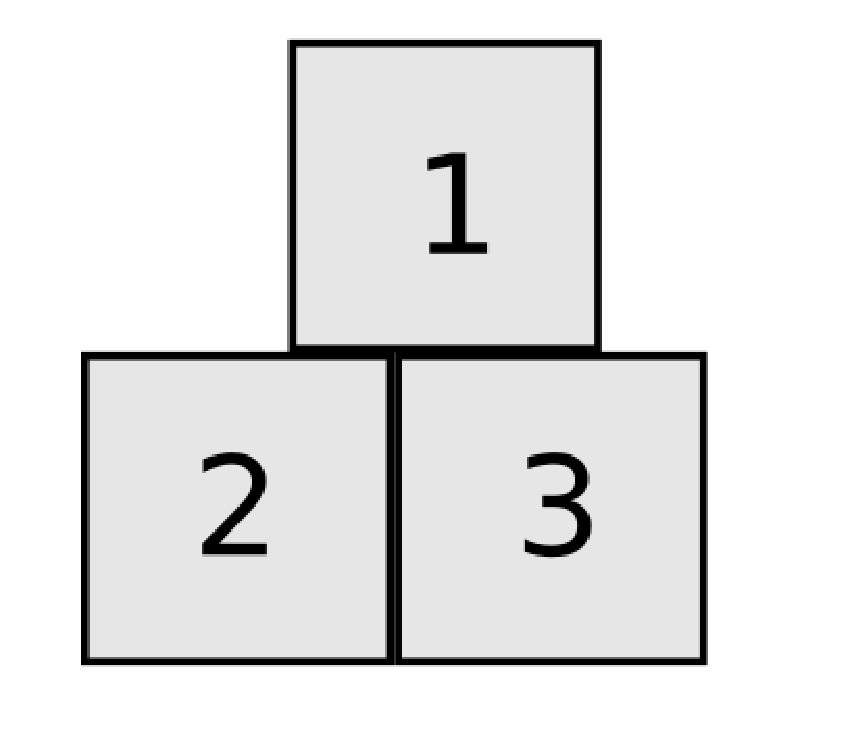
\includegraphics{figures/alignedBlocks.pdf}}
\caption{}
\end{figure}

\begin{figure}[H]
\label{fig:pythagoras}
\scalebox{.3}{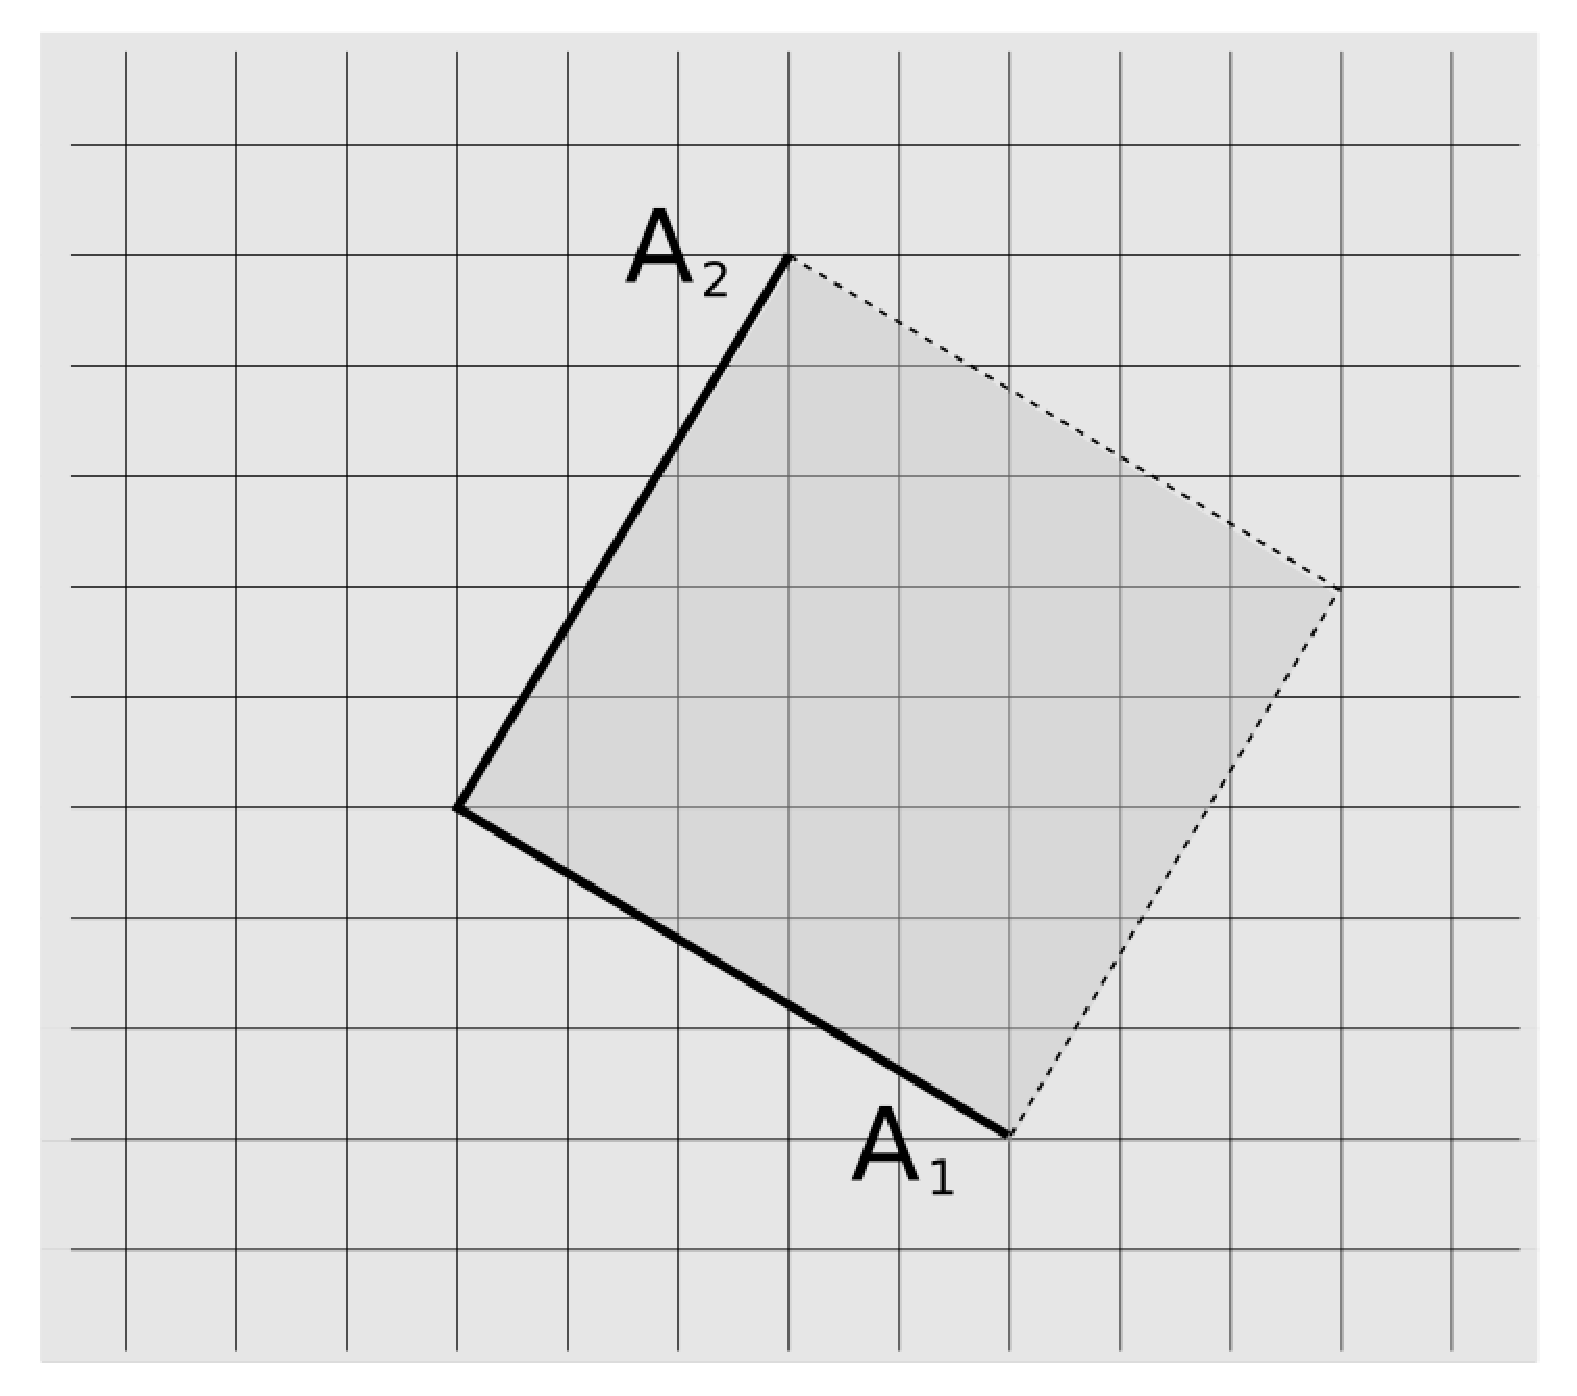
\includegraphics{figures/pythagoras.pdf}}
\caption{}
\end{figure}


\begin{figure}[H]
\label{fig:Bezout}
\scalebox{.3}{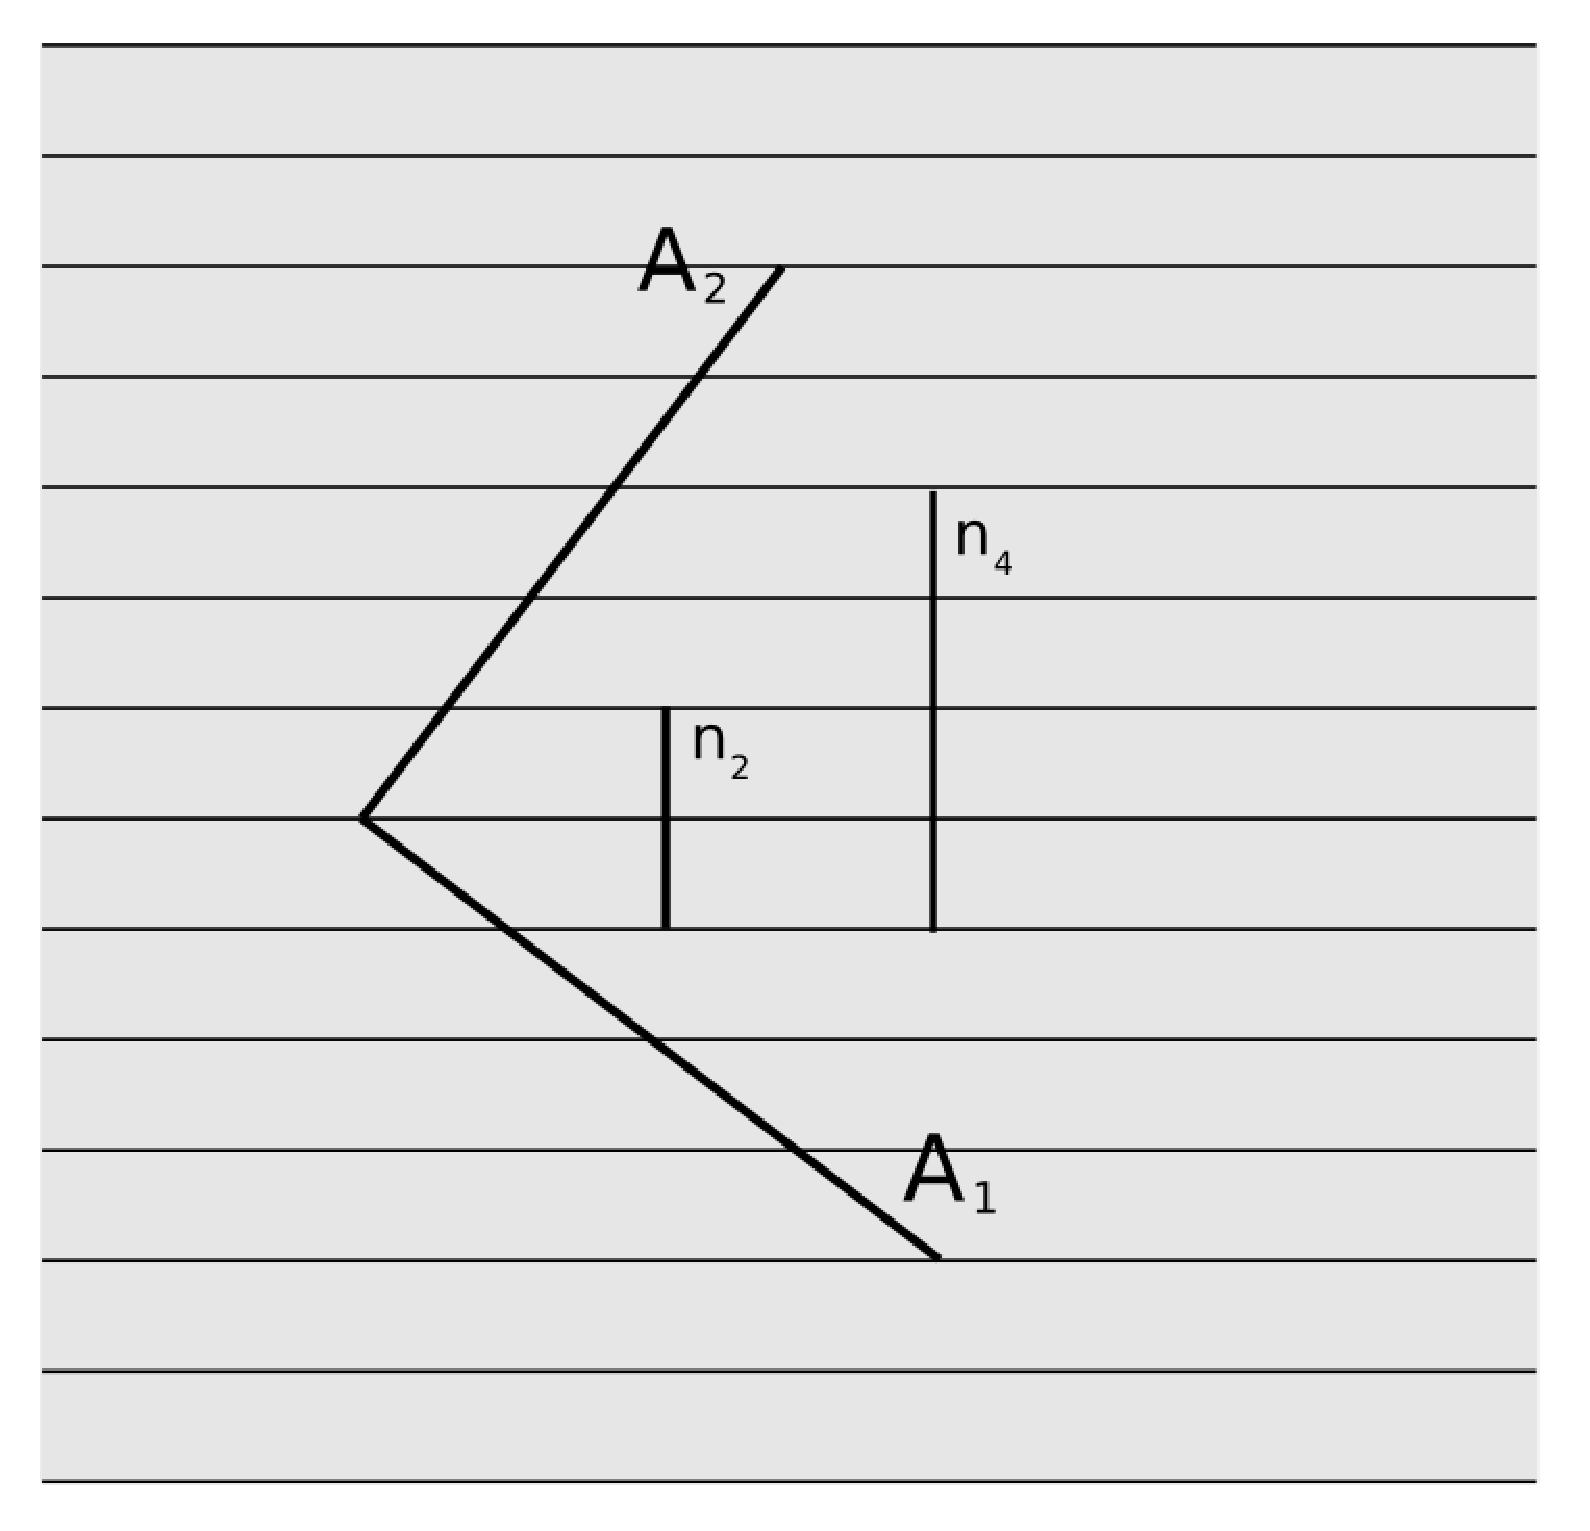
\includegraphics{figures/Bezout.pdf}}
\caption{}
\end{figure}

\section{Numerical Methods}
\label{sec:numerical}

%\subsection{New Mat}
%\subsection{Overview}
%Rintoul and Torquato, ``Computer Simulations of dense hard-sphere systems'' \cite{Rintoul1996a}
For all $N \leq 27$ squares on the flat torus, we searched for densest packings of $N$ squares on the torus via Monte Carlo simulations in the NPT ensemble.  Our approach was to perform simulated annealing (SA), in which the system was taken from an initial, low-pressure, easy-to-equilibrate state to a final, high-pressure state via an annealing schedule consisting of a series of steps in inverse pressure.  Between each pressure increase, a Metropolis algorithm appropriate to the hard square NPT ensemble was used to equilibrate the system.  Although SA quickly falls out of equilibrium at higher pressures as the energy landscape becomes rough, it appears to be an an effective algorithm for finding ground states of the system.  

%Population annealing: \cite{Hukushima2003}

%We used two related approaches to finding ground states: simulated annealing (SA) [REF??] and population annealing (PA) \cite{Machta2010a}.  SA and PA are Monte Carlo techniques that can been used to find ground states of systems with rough energy landscapes and multiple metastable states.  In both SA and PA, the system is taken from an initial,  low-pressure, easy-to-equilibrate state to a final, higher-pressure state via a series of steps in inverse pressure -- an annealing schedule. Between these pressure increases, an equilibration procedure -- in our case, a Metropolis algorithm appropriate to a hard-particle NPT ensemble, described in Section [??] -- is used in an attempt to equilibrate the system.  In SA, the system quickly falls out of equilibrium at higher pressures as the energy landscape becomes rough; nevertheless, SA remains an effective algorithm for finding ground states of a system, and is used widely in [examples].  PA [Machta and Ellis REF, Machta REF] is a way of keeping the system close to equilibrium by adding an additional step to the annealing procedure.  In PA, a collection of identical systems, or replicas, are simulated in parallel.  As in SA, all replicas are taken through a compression schedule; but in PA, after each compression, the collection of replicas is 'resampled':  some replicas are copied, and others are destroyed, in order to achieve a distribution of replica volumes that approximates the expected equilibrium Boltzman distribution at the current pressure.  Details of this procedure are described below in section [??].  We simulated several replicas using both SA and PA, and took the highest density configuration for a given $N$ found using either procedure as our best candidate for the ground state of the system.

%\subsection{Algorithm Details}
The equilibration procedure we used in our simulated annealing algorithm was a Metropolis procedure consisting of three types of Monte Carlo moves:  translations and rotations of individual squares, and changes in the volume of the entire system.  At each step of the equilibration procedure, a square is selected at random, and then one of the three types of moves is selected at random, with probabilities .495, .495, and .01 for translation, rotation, and volume change, respectively.  Once a square and a move type is selected, the move is attempted.  If the move results in any overlaps among the $N$ squares, the move is rejected.  If it does not, then for translations or rotations, the move is accepted; for volume change $dV$, the move is accepted with probability $p_{acc}=\min[1,\exp(-\beta P dV)]$.  In practice, rather than changing the volume of the entire system, the periodic box in the simulations was kept at a constant size, and the sizes of the individual squares were all rescaled, in order to achieve the desired new volume. The equilibration procedure consists of $s$ such Monte Carlo steps; in our simluations, $s$ was typically between 200 and 400 steps.  

We repeated this simulation 1,000 times, and reported the highest density found among these runs.  In order to determine the highest-density packing for $N$ that did not correspond to a perfect square or a sum of squares, more extensive runs were conducted -- as long as 72 hours on a 2GHz processor in some cases.  The fact that significantly different initial configurations and different initial random seeds generated the same final, high-density configurations signalled that we had found a good candidate for a densest packing of the system.  For all simulations, the pressure was initially set to $\beta P=.01$ and was increased via constant steps in inverse pressure until a maximum pressure of $\beta P_{max}=3000$ was reached. (During subsequent explorations of the phase behavior of the system, this pressure was later deemed excessive; but nevertheless produced reasonable results for the purposes of determing the ground state of the system.) All simulations were begun at an initial areal density $\rho$ of 0.1 with a square array of unit squares. Before each equilibration procedure began, a trial run was conducted in which the maximum value of translations, rotations, and volume changes were independently optimized in order to achieve an acceptance ratio for each of $0.4$. 

The majority of the computational work during the equilibration procedure consisted in checking for square overlaps.  For this, we relied on a fast algorithm for detecting polygon overlaps by Alan Murta [REF], and an associated Python wrapper by Joerg Raedler [REF].
%the General Polygon Clipping Library by Alan Murta (http://www.cs.man.ac.uk/~toby/alan/software/), and the Python wrapper written for this by Joerg Raedler (http://www.j-raedler.de/projects/polygon/).

Configurations were visualized using the VPython library (http://vpython.org/).


%\subsubsection{Population Annealing}

%As described above, SA consisted in taking a system (or several replicas of a system) through an annealing schedule of constant steps in inverse pressure, followed by $s$ equilibration moves after each pressure increase, until reaching a pressure at which the density appears to plateau. PA also involvs constant steps in inverse pressure, but after each pressure increase from the current pressure $P$ to the new pressure $P'$, the collection of $R$ replicas is 'resampled' so that the number of copies of a replica $j$ in the population reflect its expected equilibrium weight in the population, $w_j=\exp[-(P'-P)V_j]$. Copies of each replica $j$ are thus made in order to approximate the expected number of copies of replica $j$ in the population, 
%\begin{equation}
%p_j=\exp[-(P'-P)V_j]/Q,
%\end{equation}

%where 

%\begin{equation}
%Q=\Sigma_{j=1}^R exp[-(P'-P)V_j]/R
%\end{equation}

%Thus the appropriate number of copies of each replica can be generated by sampling from the multinomial distribution using $R$ trials [REF].  This is accomplished via a simple algorithm [REF, wikipedia, Multinomial Distribution ]: 


%\begin{enumerate}
%\item Initialize: $Q$
%\item For $i$ in range $(0,R)$:
%\begin{enumerate}
%\item $p_i=exp[-(P'-P)V_i]$
%\item $Q=Q+p_j$
%\end{enumerate}
%\item For $i$ in range $(0,R)$:
%\begin{enumerate}
%\item $p_i=p_i/Q$
%\item $X_i=\mathcal{R}(0,1)$
%\end{enumerate}
%\item Sort $X$ in ascending order
%\item Initialize: $p_{sum}$, TempReplicas, and $C$
%\item For $i$ in range $R$:
%\begin{enumerate}
%\item $p_{sum}=p_{sum}+p_i$
%\begin{enumerate}
%\item While ($C<R$) and ($p_{sum} \ge X_i$) do:
%\begin{enumerate}
%\item $C=C+1$
%\item TempReplicas[count]=Replica[i]
%\end{enumerate}
%\end{enumerate}
%\end{enumerate}
%\item For $i$ in range $(0,R)$:
%\begin{enumerate}
%\item Replica[i]=TempReplica[i]
%\end{enumerate}
%\end{enumerate}

%Where $\mathcal{R}(0,1)$ is a random number between $0$ and $1$.

%$\underset{x}{\operatorname{argmax}} $

% 1. Sort the replicas in descending order by volume; 2. For i in range(0,R):pick a random number $X$ from (0,1); choose replica $j= arg min (j'=1 to k) (\Sigma p_i >= X)$ to replace replica $i$ with a copy of replica $j$.  


%\begin{pseudocode}{Repopulate}
%\FOR i \GETS 0 \TO R \DO
%test of this line\\
%test of this line
%\end{pseudocode}

%\subsection{Results}

%A detailed analysis of the configurations found via simulation is found in Section~\ref{sec:analytics}.  For both SA and PA, our Monte Carlo simulations yielded a collection of replicas of varying densities at each pressure.  As the simulations for each $N$ progressed, we selected the highest-density configuration at each pressure using SA or PA as the candidate ground state for that $N$; the highest density reached in this manner was our best candidate for a ground state for $N$.  In Figure [?], we plot density $\rho$ vs. pressure $P$ for $N=12$ using both SA and PA.  This plot highlights a general trend:  for all values of $N$, the highest density among the PA replicas initially increased faster than that among the SA replicas at a given pressure.  In some cases (exemplified in Figure [?]), SA eventually overtook PA in density, finding a higher density configuration than any reached by PA; in others, PA found the highest-density configuration.  Figure [?] shows a simulation run for which the densities of both SA and PA had plateaued at nearly identical densities, and the associated configurations of each highest-density replica.  [SOME WORDS HERE RE: HOW EXTENSIVE OUR SIMULATIONS WERE IN CPU HOURS, HOW MUCH OF PARAMETER SPACE WE EXPLORED, AND HOUR HIGH CONFIDENCE THAT WE HAVE FOUND THE GROUND STATES FOR $N \leq 27$.  For some configurations (mentioned in Section~\ref{sec:analytics}), the ground state quickly approached density = 1 (for $N$ equal to a perfect square, e.g. 4, 16; or for $N$ equal to a sum-of-squares, e.g. 7, 10), and were provably optimal packings for that $N$; for other configurations, we are constrained merely to report our highest-density configuration as the best candidate thus far for a ground state for that $N$. In particular, the densities for $N=12,21,23$ consistently plateaued at their reported final values across several runs, and resulted in configurations that display obvious symmetry but are not necessarily ground states of the system. Results for various $N \leq 27$ are characterized in Section~\ref{sec:analytics}.

%\section{Analysis of Packings}
\label{sec:analytics}

In this section we give an analytic treatment of square packings on a torus.  We first describe a set of solutions in which the squares lie on a Bravais lattice, and then turn to more complicated cases. The density one solutions are optimal by construction, and all of the other solutions are conjectured to be optimal. The numerical results of Sec. \ref{sec:numerical} guided us to the conjectured solutions, and the fact that long simulated annealing runs consistently produced these solutions gives us some confidence that they are optimal.  Our conjectures for the first 27 values of the number of squares are summarized in Table \ref{table}.

\subsection{Commensurate Bravais Lattice Solutions}
Here we consider a class of Bravais lattice configurations that includes all of the density one packings and other solutions we have found for  $N \leq 27$.   In all of these packings the squares are lined up in rows.  For the purpose of this analysis, we assume these rows are aligned along the x-axis. Thus one of the primitive vectors of the lattice of squares is $\ax=\hat{{\bf x}}$.   The second primitive vector is taken to have the form $\ay=c \hat{{\bf x}} + d \hat{{\bf y}}$ with $-1< c <1$ and  $d\geq 1$.  The primitive vectors of the torus, $\Ax$ and $\Ay$, need not be aligned with the primitive vectors of the squares.     The requirement that the squares pack periodically on the torus is equivalent to saying that the lattice of squares is commensurate with the larger square lattice of the torus.  That is, there exist  integers $n_1$, $n_2$, $n_3$ and $n_4$ such that the torus primitive vectors $\Ax$ and $\Ay$ are given by
\begin{eqnarray} 
\label{eqn:Ana}
\Ax&=& n_1 \ax + n_2 \ay \nonumber \\ 
\Ay&=&n_3 \ax + n_4 \ay.
\end{eqnarray}
In addition, we require that the torus primitive vectors are of equal length,
\begin{equation}
\label{eqn:normal}
|\Ax|=|\Ay| ,
\end{equation}
and orthogonal,
\begin{equation}
\label{eqn:ortho}
\Ax \cdot \Ay = 0 .
\end{equation}
[ COMMENTS? ] [ HOW DO WE RECONCILE C>0 WITH FINITE ENTROPY OF PERFECT SQUARE PACKING?]
These conditions are uniquely solved by
\begin{eqnarray}\label{eq:gap}
c &=& - \frac{n_1 n_2 + n_3 n_4}{n_2^2 + n_4^2}\\
d &=& \frac{| n_1 n_4 - n_2 n_3|}{n_2^2 + n_4^2} \nonumber
\end{eqnarray}
The number of squares $N$ packed on the torus is the number of lattice points of the squares lattice in a unit cell of the torus lattice
\begin{equation}
\label{eqn:N}
N = |n_1 n_4 - n_2 n_3|,
\end{equation}
and the areal density of the squares $\rho$ is given by
\begin{equation}
\label{ }
\rho=N/|\Ax \times \Ay| = 1/d.
\end{equation}

\subsubsection{Density one packings}
There are two classes of density one solutions.  The first is the perfect square packing.  Here $c=0$, $d=1$, $n_1=n_4=\sqrt{N}$ and $n_2=n_3=0$.  This simple packing is shown in Fig. \ref{fig:N9} for the case of $N=9$.  Note that on the torus, each of the $n_1$ rows (or columns, but not both) may be arbitrarily displaced relative to the other rows (columns) without disturbing density of the packing or its periodicity.  Thus, the perfect square packings have finite entropy.

There is a more general class of density one packings for which the lattice of squares may be tilted with respect to the primitive vectors of the torus. Setting $d=1$ and $c=0$ in Eq. (\ref{eq:gap}), we find $N=n_2^2 + n_4^2$, $n_1=-n_4$, and $n_2 = n_3$.  The perfect square solution is the special case $n_2 = n_3 = 0$, with the square lattice oriented at an angle of $\tan^{-1}(n_2/n_1)$ relative to the torus lattice vectors.   Clearly, these density one, tilted square lattice solutions are optimal for all $N$ that are sums of two square integers.  Fig. \ref{fig:bravais} shows the case $N=10$ ($n_1=3$ and $n_2=1$).

The packing has density one if and only if $N$ is a sum of two squares; and the converse of this is also true: $N$ is a sum of two squares whenever we have a density one packing of squares in the torus. To prove this, first note that every square in a $\rho=1$ packing must have at least four other squares bordering it along a finite segment length, forcing all $N$ squares to share the same orientation.  Now consider three squares in mutual contact with each other, a configuration that must exist if the packing has no gaps. Two of those squares must be aligned in a row, as shown in Fig. \ref{fig:aligned}. In order to eliminate gaps in the packing, those three squares define a set of rows that the entire packing must respect. The periodicity of periodic boundary conditions on a set of rows now ensures that $N$ can be [????] expressed as $n_2^2 + n_4^2$ via the Pythagorean theorem (see Fig. \ref{fig:gb}).

\subsubsection{Density one packings with defects}

The simplest way to produce candidates for a densest packing for $N=n_2^2 + n_4^2$ is to remove $k$ squares from a density one packing; indeed, our numerical results suggest that for several values of $N$, the optimal packing is a density one packing configuration with one missing square.  This is indicated in the `Comment' column in the Table using the notation $n_1^2-k$ or $n_1^2+ n_2^2-k$ depending on whether they are generated by removing $k$ squares from $N$ a square integer or a sum of two square integers respectively. Examples include $N=3$, $7$ and $15$. Note that these configurations have finite entropy since the hole(s) in the lattice can be distributed arbitrarily.

[ should the notation $n_1^2-k$ or $n_1^2+ n_2^2-k$ include a -1??? or ...? For $N \leq 27$, $k=1$] (see jon's edits]

%Although for small $N$, the density of sums of two squares together with perfect squares is relatively high,  it is known RAMANUJAN ETC REFERENCE that these values of $N$ have vanishing density among all positive integers. In particular the density of sums of two squares less than $n$ behaves asymptotically as $1/\sqrt{\log(n)}$. One interesting consequence of this is that $\rho=1$ packings appear with vanishing frequency as $N  \rightarrow \infty$. 

%Unlike the perfect square packings, the sum of two squares packing must have all the rows of squares aligned and do not have finite entropy.

\subsubsection{Bricklayer packings with gaps}
Next we consider Bravais lattice solutions that have density less than one -- that is, $d>1$.  Because these solutions may also have rows that must be shifted relative to one another ($c\neq 0$), we call these `gapped bricklayer configurations.'  An example is shown in Fig. \ref{fig:gb}(a).  The equations of (\ref{eq:gap}) allow us to ennumerate all gapped bricklayer configurations. Since the packing density of these configurations is $(n_2^2 + n_4^2)/N$, the highest packing density we can find within this class of configurations with density less than unity must numbers of the form $n_2^2 + n_4^2 = N-1$.  This requires that $N$ be one more than a sum of two squares. The first several are 2,3,6,11,14,18,26, and 27.  Based on the numerics we believe that for $N=6$, 11, 14 and 27, the gapped bricklayer packing is optimal. These are indicated in the Table with the abbreviation `GB' in the Comment column. The associated (not unique) lattice vectors are shown in the rightmost columns of the Table for the GB packings.  There are also gapped bricklayer solution for density $(N-2)/N$ when $N$ is two more than a sum of two squares though we have not found any candidate optimal solutions of this form for $N \leq 27$. Unlike the bravais lattice packings with density one, different rows of the gapped bricklayer solutions have a fixed shift given by $c = - (n_1 n_2 + n_3 n_4)/(n_2^2 + n_4^2)$. The denominator is the closest sum of two squares below $N$. 

\subsection{Non-Bravais Lattice Packings}

Here we consider special cases suggested by our numerical simulations that do not correspond to Bravais lattice packings.
Note: if the 'Comment' column of the Table simply repeats a value of $N$, it indicates a special case for which the squares are not on a Bravais lattice and for which there is not an obvious pattern that can be extrapolated easily to optimal packings for higher values of $N$.

\subsubsection{Gapped bricklayer with domino bricks, $N=22$}
The conjectured best packing for $N=22$ is shown in Fig. \ref{fig:n22} It is actually a gapped bricklayer configuration except that the unit cell or brick is composed of two squares stacked in the $\hat{{\bf y}}$ direction (the direction perpendicular to the rows).  Except for this difference, the configuration is identical to the $N=11$ gapped bricklayer and has density $\rho= 10/11$.

\subsubsection{Lattice of $\frac{1}{2}\times\frac{1}{2}$ holes, $N=12$ and $23$}
The conjectured best configurations for $N=12$ and 23 are shown in Figs. \ref{fig:n12} and \ref{fig:n23}, respectively.  In both cases the motif can be described as a lattice of $\frac{1}{2}\times\frac{1}{2}$ holes. It is straightforward to verify that these motifs are in fact packings on the torus and have the density $N/(N+k/4)$ where $k$ is the number of holes in the unit cell.  For $N=12$, evidently $k=2$ and for $N=23$, $k=5$. 


\subsubsection{Lattice of skew squares embedded in a square lattice, $N=21$}
The conjectured densest packing for  $N=21$, shown in Fig.\ \ref{fig:n21}, does not follow any of the motifs described heretofore. The unit cell consists of a $4 \times 4$ square with motif of 5 squares attached to its side.  This 5-square pattern is also the best packing of 5 squares in a square \cite{Friedman2002}.  A simple calculation yields the density, $\rho= 21/(4^2+(2+1/\sqrt{2})^2)$.  This packing has one square per unit cell tilted at 45$^{\circ}$ relative to all other squares.  This is the only example that we found for which not all of the squares in the motif are oriented in the same way. It was also the most difficult configuration for our simulated annealing algorithm to find. 

\subsection{Table of Results}

To summarize: the perfect square, sum of two squares and gapped bricklayer configurations cover most of the case we have found for $N \leq 27$.  The Table gives optimal configurations (if $\rho=1$) and conjectured optimal configurations (if $\rho<1$), for each value of  $N$ less than 28.  The column `$\rho$' is the density of the configuration. The `Comment' column describes the type of lattice.   For example, $3^2$ indicates a perfect square and $5^2-1$ indicates a perfect square with one square missing.  Similarly $3^2+1^2$ refers to the sum of two squares and `GB' stands for `gapped bricklayer.'  If a single number is in the `Comment' column it refers to one of the special cases discussed above.  The four columns `$n_1$, $n_2$, $n_3$, $n_4$' are shown if the configuration of squares is itself a Bravais lattice and these integers are the coefficients of the lattice vectors of the torus in terms of the lattice vectors of the squares as defined in (\ref{eqn:Ana}).  Only those columns needed to specify the lattice are filled in.

\vspace{.3in}
\begin{table}
\label{table}
\caption{Exact and conjectured densest packed configurations of squares on a torus.  Refer to the text for the meaning of the columns.}
  \begin{tabular}{|c | c|c | c| c | r | c | c | c |}
\hline
% after \\ : \hline or \cline{col1-col2} \cline{col3-col4} ...
  $N$ &$\rho$&Comment& $n_1$ & $n_2$ & $n_3$ & $n_4$  \\ \hline \hline
   1 &1&  $1^2$ & 1&  &   &    \\ \hline 
   2 &1&  $1^2+1^2$ &1& 1 &  &  \\ \hline
   3 &$3/4=0.75$&  $2^2 -1$ &2&  & &   \\ \hline
   4 &1&  $2^2$ &2& & &   \\ \hline
   5 &1&  $2^2+1^2$ &2& 1 &    & \\ \hline
   6 &$5/6=0.8\bar{3}$& GB &2& -1 &2 & 2   \\ \hline
   7 &$7/8=0.875$& $2^2+2^2 -1$ &2& 2 & &     \\ \hline
   8 &1& $2^2+2^2 $ &2& 2 & &     \\ \hline
   9 &1&  $3^2$ &3& & &  \\ \hline
   10 &1&  $3^2+1^2$ &3& 1 &    & \\ \hline
   11 &$10/11=0.\overline{90}$& GB &3& 1 &-2 & 3   \\ \hline
   12 &$24/25=0.96$& 12 && & &    \\ \hline
   13 &1&  $3^2+2^2$ &3& 2 &    & \\ \hline
   14 &$13/14=0.9\overline{285714}$& GB &3& 2 &4 & 2   \\ \hline
   15 &$15/16=0.9375$&  $4^2 -1$ &4&  & &   \\ \hline
   16 &1&  $4^2$ &4& & &   \\ \hline
   17 &1&  $4^2+1^2$ &4& 1 &    & \\ \hline
   18 &1&  $3^2+3^2$ &3& 3 &    & \\ \hline
   19 &$19/20=0.95$&  $4^2 +2^2 -1$ &4& 2 & &   \\ \hline
   20 &1&  $4^2+2^2$ &4& 2 &    & \\ \hline
   21 &$21/(4^2+(2+1/\sqrt{2})^2)=0.900189 \ldots$&  $21$ & &  &   &    \\ \hline 
   22 &$10/11=0.\overline{90}$& 22 &3& 1 &-2 & 3  \\ \hline
   23 &$92/97=0.94845 \ldots$&  $23$ & &  &   &    \\ \hline
   24 &$24/25=0.96$&  $5^2 -1$ &5&  & &   \\ \hline
   25 &$1$&  $5^2$ &5&  & &   \\ \hline
   26 &1&  $5^2+1^2$ &5& 1 &    & \\ \hline
   27 &$26/27=0.\overline{962}$& GB &4&3 &-5 & 3  \\ \hline

\hline
\end{tabular}
\end{table}





\section{Discussion}
\label{sec:discussion}


In this section we discuss the density and entropy of various of the packings discussed above. 

\subsection{Frequency of $\rho=1$ as $N \rightarrow \infty$}

We showed in Section XX [???] that $\rho=1$ packings are only possible for those values of $N$ that are expressible as the sum of two squares. 
%First, it is clear that all density one packings must be arranged in rows: every square in a $\rho=1$ packing must have at least four other squares bordering it along a finite segment length, thus forcing all $N$ squares to share the same orientation.  Then it is clear that for such oriented configurations, all of the squares must be arranged in rows, since for any three squares that touch one another and are oriented in the same direction, two of out of the three squares must define a row. Finally: if all squares for $\rho=1$ packings are thus arranged in rows, the periodicity requirement of toroidal boundary conditions ensures that the number of squares $N$ in the packing can be expressed as $N=n_1^2+n_2^2$, via the Pythagorean theorem (see Figure \ref{fig:pythagoras}).  In this way, we see that $\rho=1$ packings are only possible when $N$ is a perfect square or expressible as a sum-of-squares; and as mentioned above, this means that $\rho=1$ appear with vanishing frequency as $N  \rightarrow \infty$.

%Table \ref{table} indicates the values of $N$ that are either perfect squares or sums of two squares.  In the Comment column of the Table these values are indicated either by the forms $n_1^2$ or $n_1^2+ n_2^2$, respectively. 
Though it appears that density one packings are relatively common from the Table, in fact we know that the frequency of numbers that are the sums of two square integers scales as $1/\sqrt{\ln N}$ for large $N$ \cite{Berndt1993} \cite{Landau1909}.
% for more references on density of sums of squares, see http://mathworld.wolfram.com/SumofSquaresFunction.html 
As a consequence of this, the frequency of density one packings also vanishes with increasing $N$.

\subsection{Density of configurations as $N \rightarrow \infty$}
Despite the relative scarcity of density one packings, a statistical argument yields $\rho \rightarrow 1$ as $N \rightarrow \infty$. We show this by first generating a lower bound on the packing density for every $N$ by simply removing squares from a nearby density one packing. More precisely, suppose $M$ is a sum of two square integers. Define a new packing for $N = M-k$ by removing $k$ squares. The resulting packing density gives a lower bound of $\rho=N/(N+k)$. Given a number of squares, $N$, however, determining $k$ requires knowledge of the nearest density one packing larger than $N$. For sufficiently large $N$, we can estimate that the distance to the next density one packing is of order $\sqrt{\ln N}$ larger than $N$. Therefore, a lower bound on the packing density of $N$ squares is $1-\sqrt{\ln N}/N$ for large $N$ which yields the result that the density approaches one asymptotically. This simple argument does not take into account fluctuations in the spacing of sums of two squares and it would be interesting to find a mathematically rigorous asymptotic lower bound on the packing density.  For squares in a square REFERENCE shows that this bound is SQUARES IN SQUARE BOUND.

\subsection{Entropy of $\rho=1$ packings}

%JM: I DID SOME EDITING OF THE FOLLOWING PARAGRAPH
The entropy of $\rho=1$ packings depends on $N$ in the following way.  Because $\rho=1$ packings must always be arranged in rows (see above), the only contribution to the entropy comes from the freedom
of row(s) to shift relative to the each other.  Thus the entropy will be proportional to the number of rows that can be  shifted independently.  In Figure \ref{fig:pythagoras} we see that the number of rows that can be shifted independently is proportional to the smallest integer that can be written in the form $g=a n_2 + b n_4$, where $n_2$ and $n_4$ are defined as above (and in Figure \ref{fig:Bezout}), and $a$ and $b$ are integers.  Bezout's Lemma \cite{Surhone} states that this integer linear combination can be made equal to, but not smaller than, $g$, where $g$ is the greatest common divisor of $n_2$ and $n_4$;  thus, the entropy of $\rho=1$ packings will be proportional to $d$.  

\subsection{Entropy of gapped bricklayer solutions}

As discussed previously in the Section XX [???], different rows of the gapped bricklayer solutions have a fixed shift given by $c = - (n_1 n_2 + n_3 n_4)/(n_2^2 + n_4^2)$. This has ramifications for the packing entropy, since we are no longer free to arbitrarily shift rows. In Fig. [??], the lattice vectors are shown on a schematic representation of a gapped bricklayer configuration. Two rows are locked with respect to each other when a linear combination of the torus primitive vectors $\mathbf{A}_1$ and $\mathbf{A}_2$ points between the two rows. In particular, if $|n_2|$ and $|n_4|$ are mutually prime, all rows are locked and the entropy of the configuration vanishes. Alternatively, the greatest common divisor of $|n_2|$ and $|n_4|$, $g=\textrm{gcd}(|n_2|,|n_4|)$, tells us that every $g^{th}$ row is locked. Thus, the entropy of a gapped bricklayer configuration is proportional to $(n_4-n_2)(1-1/g)$.  

[INCLUDE DISCUSSION OF ``poor workmanship'' entropy of GB and refer to figure 3B]

\subsection{Rotational invariance of $\rho=1$ packings as $N \rightarrow \infty$}

Unlike squares packed into a square boundary, squares packed on a torus maintain rotational invariance in the thermodynamic limit.  This can be seen as follows: one can see in Figure \ref{fig:pythagoras} that any $N=n_1^2+n_2^2$ packing (which are, as seen above, the only possible packings for $\rho=1$) will orient the square lattice at an angle of $\tan^{-1}(n_2/n_1)$ relative to the torus lattice vectors.  One may approach the thermodynamic limit $N \rightarrow \infty$ by choosing a particular subsequence of integers $N_i=n_{1,i}^2+n_{2,i}^2$ such that 
%JM: I MADE THIS A STATEMENT ABOUT THE LIMIT AND REMOVED THE NOTE
$\frac{n_{1,i}}{n_{2,i}} \rightarrow r$; and the constant $r$ will thus pick out some particular orientation of the square lattice with respect to the underlying torus 
%(note that if $r$ is irrational, the ratio $\frac{n_{1_i}}{n_{2_i}}$ approaches, but never equals, $r$). 
Thus the thermodynamic limit of $\rho=1$ packings on the torus  preserves orientational symmetry.

\subsection{Concluding remarks}

Our study of the densest packings of $N$ unit squares in a torus has yielded definitive results for cases in which $N$ is the sum of two square integers or is a perfect square, and strong conjectures for other values of $N \le 27$.  The NP-hard status of this problem suggests that a pattern in the configurations for general $N$ will necessarily remain elusive.  In addition, several other questions arise, including: Are there finitely or infinitely many $N$ for which not all squares have the same orientation? Are there other best packings on a torus that include non-trivial packings in the square?

\documentclass[preprint,aps]{revtex4}
\newcommand{\ax}{{\bf a}_1}
\newcommand{\ay}{{\bf a}_2}
\newcommand{\Ax}{{\bf A}_1}
\newcommand{\Ay}{{\bf A}_2}

%\usepackage{graphicx}

\begin{document}
\title{Packing Squares in a Torus: Figures}

\author{D. Blair}
\email[]{dwblair@physics.umass.edu}
\affiliation{Department of Physics,
University of Massachusetts,
Amherst, MA 01003-3720, USA}

\author{J. Machta}
\email[]{machta@physics.umass.edu}
\affiliation{Department of Physics,
University of Massachusetts,
Amherst, MA 01003-3720, USA}
\affiliation{Santa Fe Institute, 1399 Hyde Park Rd, Santa Fe, NM 87501, USA}

\author{C. Santangelo}
\email[]{santangelo@physics.umass.edu}
\affiliation{Department of Physics,
University of Massachusetts,
Amherst, MA 01003-3720, USA}

\begin{abstract}
abstract
\end{abstract} 
\maketitle

\begin{figure}
\scalebox{.12}{\includegraphics{N0011population.pdf}}
\caption{Population:\\ $d=0.908798$}
\end{figure}


\end{document}


  
\bibliographystyle{apsrev}
\bibliography{squares}

\begin{acknowledgements}
We would like to thank James Hanna and Narayanan Menon for useful discussions of some of the issues addressed in this paper.  J.M. gratefully acknowledges support from a National Science Foundation grant DMR-0907235. C.S. gratefully acknowledges support National Science Foundatoin grant DMR-0846582. D.B. is grateful for use of the Hoffman2 computing cluster at UCLA.
\end{acknowledgements}

\end{document}

 
